\startchapter{Background}
\label{chapter:background}

\section{IEEE 802.11ah Standrad}

 The IEEE 802.11ah standard is one of the recent standards by IEEE organization. This standard introduces many new concepts for the first time, including new designs for both physical and MAC layer. The 802.11ah standard has been designed with three use cases in mind, smart sensors, back-haul aggregation and extended range hot-spot. In smart sensor use case, 802.11ah is designed to handle a very large number of nodes (up to 6000) connected to one access point. In the back-haul use case, an 802.11ah access point is designed to be used as an aggregator for wireless personal area network (WPAN) devices that use IEEE 802.15.4.g standard. WPAN (802.15.4g) devices have small transmission range and data rate, so in this case, 802.15.4g routers, gather data from 802.15.4g devices and send them to a single 802.11ah aggregator. In the extended hot-spot use case, 802.11ah access points can be used as candidates for cellular offloading, specially in outdoor environment where other .11 standards suffer from their short range.

\subsection{Physical Layer of IEEE 802.11ah}
In the Physical Layer (PHY), 802.11ah makes use of sub 1GHz license-exempt bands. This is the main physical layer difference between this standard and previous .11 standards. Also, 802.11ah mostly focuses on small bandwidths and does not allow $>$20 MHz bands. The use of smaller carrier frequency gives 802.11ah a much larger transmission range compared to other .11 standards. In outdoor scenarios, using default transmission power (200mW), 1MHz channel and Modulation and Coding Scheme (MCS) 10, it can achieve a range as high as 1 km \cite{khorov2015survey}. 

\subsection{Medium Access Control layer of IEEE 802.11ah}
 In the Medium Access Control (MAC) layer, 802.11ah introduces may new concepts from shortened frame formats to channel access and power management. In the main 802.11 standard, the number of nodes that can be connected to one access point is limited to 2007. IEEE 802.11ah extends this range to 8191 nodes to support the smart sensor use case. Also to better support dense network scenarios, 802.11ah shortens the length of frame headers, control frames such as ACKs and periodically transmitted frames such as beacon messages. The main change in 802.11ah which is also the focus of this thesis are changes in the channel access. 

 In order to handle the large contention between nodes in dense scenarios, 802.11ah divides all nodes connected the access point into different groups, each group is then given a specified time window called Restricted Access Window (RAW) to use the wireless channel while members of all other groups remain silent. This essentially divides the beacon period into multiple RAWs each dedicated to one group. It not only decreases the contention that one node experiences while using the wireless channel, also lets nodes save power by going to sleep in RAWs that do not belong to them. It is left to the access point to decide whether or not to allow nodes to cross the RAW boundary just to finish an ongoing transmission (Cross Slot Boundary). This channel access mechanism is called Group Synchronized Distributed Coordination Function (GS-DCF) which is to be used instead of the traditional DCF.   

\section{The Hidden Terminal Problem}
\begin{figure}
  \centering
  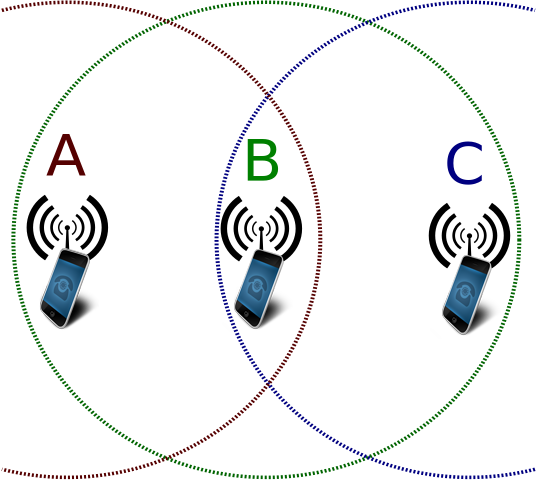
\includegraphics[width=.65\textwidth]{figures/hidden}
  \caption{A simple illustration of hidden terminal problem}
  \label{fig:hidden}
\end{figure}

The hidden terminal is a traditional problem in wireless communications. It usually happens when a node falls outside of sensing area of another node but they are both trying to communicate with a same node. Figure \ref{fig:hidden} illustrates a general case for the hidden terminal problem. For example, if the node A, first start the transmission of a packet to node B, and sometime in the middle of their communication, node C also decides to transmit a packet to B, according to the Carrier-Sense Multiple Access with Collision Avoidance (CSMA/CA) procedure, used in many wireless MAC layers, it will first listen to the channel, and since it can not sense the signal coming from A, it will find the channel ideal and initiate its transmission to B which will result in collision at B and loss of both packets of A and C. Wireless LANs in the infrastructure mode considering the up-link transmission, where every other node wants for transmit to the access point, are vulnerable to this problem. 


The legacy solution for this problem is the use of Request To Send (RTS) and Clear To Send (CTS) messages. Using these messages, every node has to send an RTS packet to its receiver and wait until it gets a CTS packet before starting a transmission. In this way, although node C might not sense the RTS from node A, it will receive the CTS that B sends to A and know that the channel for B is going to be busy. The only chance of collision because of the hidden terminal then, is during the transmission of the RTS message. Since the RTS is a small control message, collision probability will be reduced significantly. 

Given the extended range of communication in the 802.11ah standard, this problem becomes even more serious.  



\section{Physical Layer Network Coding}

The concept of Network Coding is nothing new in the wireless domain. It relies on optimizing transmission of data by combining two or more messages in a network. Physical Layer Network Coding(PNC) is then nothing but a network coding happening at the physical layer.

We use a three node linear network example to illustrate this idea \cite{zhang2006hot}. In figure \ref{fig:justThreeNodes}, nodes $A$ and $B$ have packets to exchange and node $R$ can act as a relay.


\begin{figure}
    \centering
    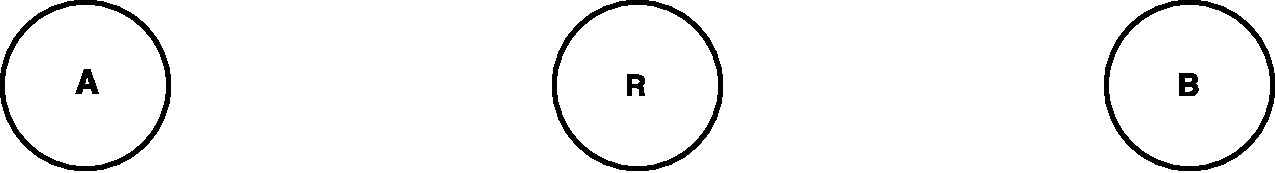
\includegraphics[width=0.8\textwidth]{figures/justThreeNodes.pdf}
    \caption{Simple three node linear network. Nodes $A$ and $B$ have packets to exchange and node $R$ acts as relay} \label{fig:justThreeNodes}
\end{figure}

Assuming that $A$ and $B$ are too far for a reliable transmission, there are different ways for this exchange of packets to happen, traditional relaying, straightforward network coding and physical layer network coding.

An exchange of packets between $A$ and $B$ where relay only works as a traditional decode and forward node takes four time slots as illustrated in figure \ref{fig:traditionalRelay}.  

\begin{figure}
    \centering
    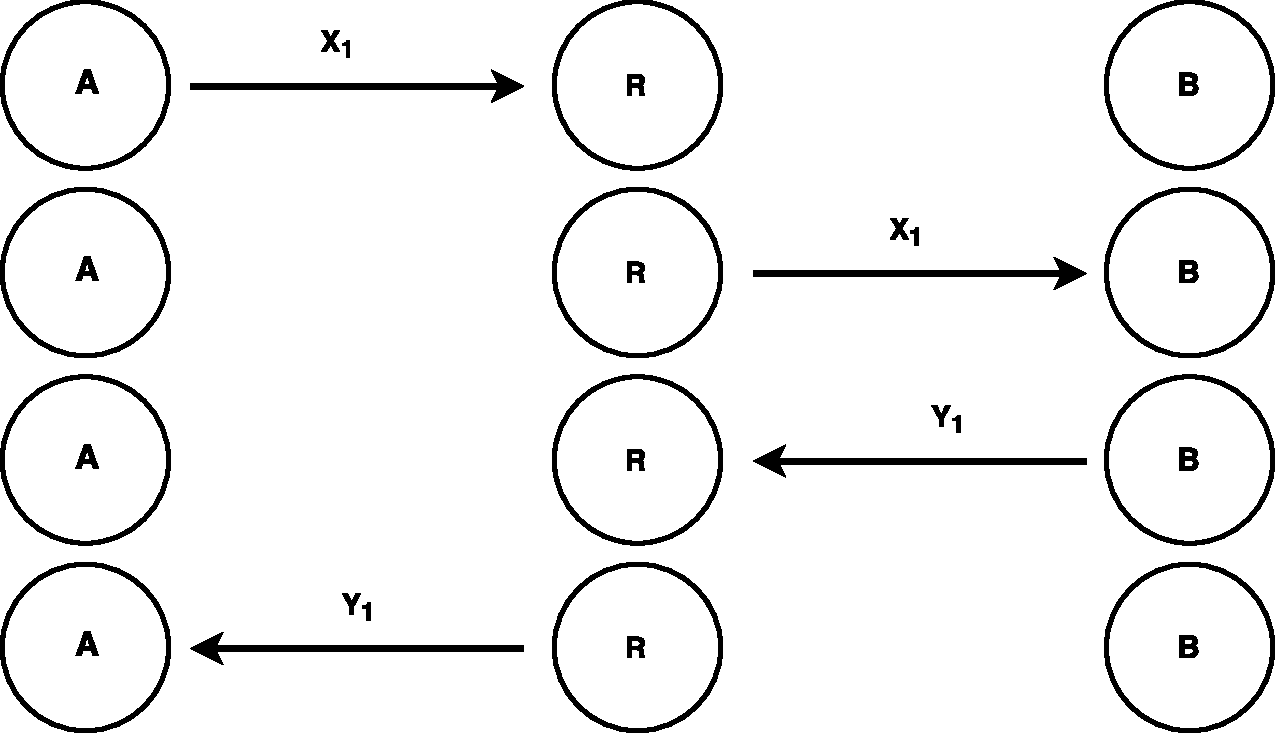
\includegraphics[width=0.8\textwidth]{figures/traditionalRelay.pdf}
    \caption{Traditional relaying. First, node $A$ transmits its packet to the relay, then the relay forwards $A$'s packet to $B$, then in time slot three, node B sends its packet to the relay, which is then forwarded to node $A$ in time slot four.} \label{fig:traditionalRelay}
\end{figure}

Using straightforward network coding, reduces the number of time slots required for that aforementioned exchanged to happen to three. Figure \ref{fig:straightforwardNC} shows this scenario. This way, using the broadcast nature of the wireless channel, the relay having stored both $A$ and $B$'s message, broadcasts a combined version of $X_1$ and $Y_1$. Then both $A$ and $B$ can decode the other node's packet, having their own message and the message they received from the relay. The simplest coding scheme to be used by relay to generate the combined message is calculating XOR of  $X_1$ and $Y_1$.

\begin{figure} 
    \centering
    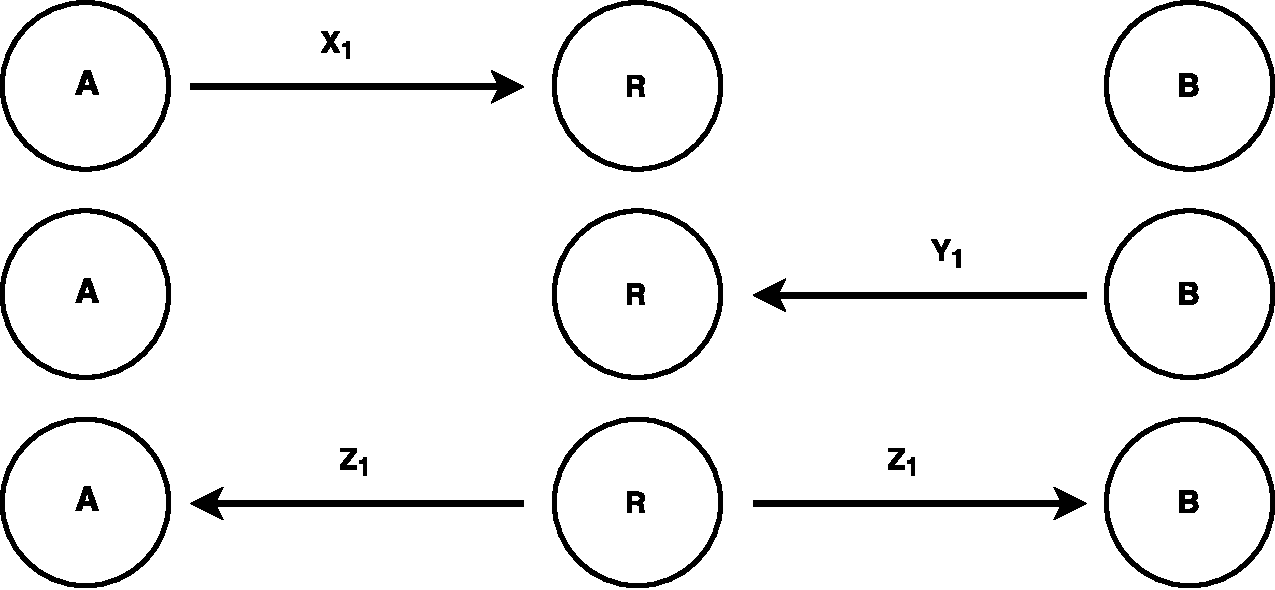
\includegraphics[width=0.8\textwidth]{figures/straightforwardNC.pdf}
    \caption{Straightforward network coding. First, $A$ transmits its packet to relay, then $B$ transmits its message to the relay, then relay calculates $Z_1=X_1 \oplus Y_1$ and broadcasts it to $A$ and $B$ in time slot three, which can then decode the other nodes message by another XOR.} \label{fig:straightforwardNC}
\end{figure}

\begin{figure}
    \centering
    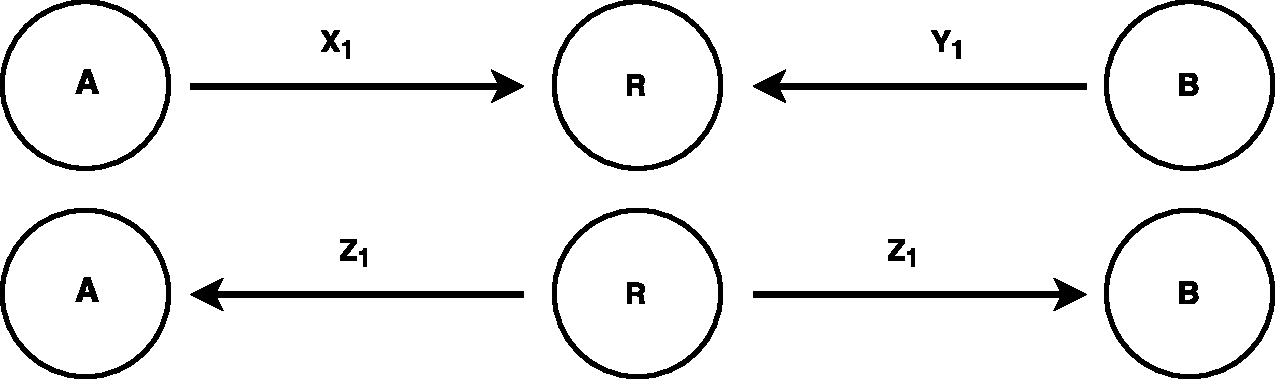
\includegraphics[width=0.8\textwidth]{figures/threeNodePnc.pdf}
    \caption{Physical layer network coding. In time slot one, $A$ and $B$ will transmit their packets to the relay at the same time (multiple access phase). The relay, using its mapping function extracts XOR of $A$ and $B$'s packets and broadcasts it to them in time slot two (broadcast phase).} \label{fig:threeNodePnc}
\end{figure}

Physical layer network coding is similar to straightforward networking coding with the difference that in PNC, the two messages from $A$ and $B$ are coded (combined) in the physical layer using the additive nature of simultaneously arriving electromagnetic (EM) waves \cite{zhang2006hot}. This reduces the number of time slots for the same exchange to happen to two. In a simple BPSK modulation where 0 and 1 are represented with $-1$ and $+1$ respectively, if $A$ and $B$ transmit their packet to the relay at the same time, they relay will received symbols of $-2$, $0$, and $+2$. At this step, every PNC capable relay requires a mapping function, to convert these new symbols into bits of data with a meaningful relationship to $A$ and $B$'s bits. In this simple BPSK example, mapping $-2$ and $+2$ symbols to 1 and $0$ symbols to 0, means that the received message at the relay is again XOR of $A$ and $B$'s packets. Just like the straightforward network coding, the relay then broadcasts this information back to $A$ and $B$ and they will use it to extract the other node's packet.

The same technique can be extended to linear multi-hop networks with more than two hops. Although a multi-hop scenario suffers from interference from other nodes, PNC is among technologies that can still maintain a reliable error rate and much higher throughput.


\section{Software Defined Radio}

Talk about SDR, GNURadio, USRP with some figures maybe.